% A good introduction to latex can be found here:
%  http://www.cse.ohio-state.edu/~hank/latex/lshort141.pdf

\documentclass{article}
\usepackage{amsmath}

\usepackage{full page}  % make the margins somewhat smaller than the default

\usepackage{listings}  %  needed for source code listings
\usepackage{color}
\usepackage{hyperref}
\usepackage{graphicx}
\usepackage[tight,footnotesize]{subfigure}

\definecolor{javared}{rgb}{0.7,0,0} % for strings
\definecolor{javagreen}{rgb}{0.25,0.6,0.35} % comments
\definecolor{javapurple}{rgb}{0.55,0,0.40} % keywords
\definecolor{javadocblue}{rgb}{0.25,0.35,0.85} % javadoc
 
\lstset{language=Java,
basicstyle=\ttfamily,
keywordstyle=\color{javapurple}\bfseries,
stringstyle=\color{javared},
commentstyle=\color{javagreen},
morecomment=[s][\color{javadocblue}]{/**}{*/},
numbers=left,
numberstyle=\tiny\color{black},
stepnumber=2,
numbersep=10pt,
tabsize=4,
showspaces=false,
showstringspaces=false,
frame=shadowbox,
numbers=left
} 

% set the document title, author, and date here.
%  once set, the \maketitle command (within the document)
%  will display them nicely
\title{Motion Planning}
\author{Junjie Guan $<gjj@cs.dartmouth.edu>$}

\begin{document}
\maketitle

\tableofcontents

\section{Introduction}

Motion planning is a very intersting problem in our realworld. One key issue here is that the metrics beacome infinite in real world, while computer can only handle finite number of states. In this report we introduce some planning methods that is able to build a search tree/graph for real world problem (here the problem is motion planning).

\clearpage
\section{Probabilistic Roadmap (PRM)}
\subsection{Basic Idea}

The basic idea of PRM is first sampling the real world and creat a finite configuration space. Then we create a search graph based on the relationship of each configuration (usually a multi-dimensional distance). Then we use traditional path searching algorithm such as A* to find a solution from the start to the goal.






\clearpage
\section{Multirobot problem}
\subsection{Problem definition and states}

The different between single robot problem and multi robot problem is, every robot take turns to make actions, and it needs collision detection. In thiscase, we decide the a whole state for all the $k$ robots, like this:



$$\begin{pmatrix}
x_0 & y_0 \\
x_1 & y_1 \\
\vdots & \vdots \\	
x_{k-1} & y_{k-1}
\end{pmatrix}$$
However, this is not enough for the states. We still one parameter, which the turn of the robot. This parameter is not necessary, which means you can still solve the problem without it in the state. However, returning all the possible states of $k$ can be very redundant and time consumming for latter searching. If I have k robot, and five actions (4 directions plus not moving), the upper bound of states would be $5^k$. It is like giving too much options more next step, while I am not making any decision.











\subsection{Discussions}
ith $n\times n$ size of maze and $k$ robots, the upper bound of this problem, meaning to neglect the legal problem, is $n^{2k}$. Because each robot has $n$ possible position.

If number of wall square is $w$, then the number of collisions would be total state minus legal states, $(n^2-w)^k - C_{n^2-w}^k$. 

As for $100\times100$, with a few walls and several robot discussion. States number grows exponentially with $k$, and bfs tends to search all the state starting from start node. I think this problem still depends on whether the goal is close to the starting point.

As for the design of heuristic, I will use the following function,
$h = \sum^{k-1}_{i=0}h_i$, where $h_i$ represents the Manhattan distance from robot $i$ to the goal. A function is monotonic as long as\footnote{from \url{wiki: http://en.wikipedia.org/wiki/Consistent_heuristic}}:

$$h(N) \leq c(N,P)+h(P) $$
$$h(G)=0$$
where

\begin{itemize}
\item h is the consistent heuristic function,
\item N is any node in the graph,
\item P is any descendant of N,
\item G is any goal node,
\item c(N,P) is the cost of reaching node P from N.
\end{itemize}

It is obvious that for single robot, the single heuristic satisfy this condtions. An extreme case is the empty maze, where $h(N) = c(N,P)+h(P) $. In any other kind of maze, due to the obstacles, the $h$ usually larger than $cost$, because Manhattan distance is the shortest distance.

Under the condition that single heuristic satisfy this condtions. Adding them together should not affect the monotonicity.

The 8-puzzle problem is the case of multi-robot where there is no walls, and there is only one free space to move, and the goal is letting each robots move to its corresponding positions.

Whether 8-puzzle can be divided into two disjoint? This is similar to graph connectivity problem, or disjoint set problem. There is no better way but to traverse through all the possible states in 8 puzzle.

Let's say the total I calculate that the total states amount of this problem is $N$. My basic idea is, first I pick an arbitrary state, and use bfs to traverse all the connected states, push every one of them into a \textbf{hash set}. At this point the number of the set should be less then $N$. (Otherwise we turn out to prove there is no disjoint set.) Then I will pick antoher state that is not blong to the first set, and also use bfs to create another \textbf{hash set}. Finally, the sum of this two set should equal to $N$.



















\subsection{Code implementation}


\subsubsection{getSuccessors}

\textbf{getSuccessors} is used to expand new states from the current state.

\textbf{Line 4:} Iterate through all the 5 possible actions (4 directions plus not moving).
\textbf{Line 6-7:} Initiate the coordinates for the successor's state, noted that only the robot in turn can take action here.
\textbf{Line 11-13:} Construct the successor with new coordinates, and new cost based on whether it moves, and also keep looping the turn through $R$ robots.

\begin{lstlisting}[numbers=left]
public ArrayList<SearchNode> getSuccessors() {
  ArrayList<SearchNode> successors = new ArrayList<SearchNode>();
  Integer[] xNew = new Integer[R], yNew = new Integer[R];
  // take actions
  for (int[] action : actions) {
    for (int r = 0; r < R; r++) {
      xNew[r] = robots[r][0] + action[0] * (r == turn ? 1 : 0);
      yNew[r] = robots[r][1] + action[1] * (r == turn ? 1 : 0);
    }
    if (maze.isLegal(xNew[turn], yNew[turn])
        && noCollision(xNew, yNew)) {
      SearchNode succ = new MultirobotNode(xNew, yNew, getCost()
          + Math.abs(action[0]) + Math.abs(action[1]),
          (turn + 1) % R);
      successors.add(succ);
    }
  }
  return successors;
}
\end{lstlisting}


\subsubsection{noCollision}

\textbf{noCollision} is used to determine whether there is a collision of robots. I set it as private seems it is not used for outter class.

The basic idea is, I hash the position of each robot, and and check if the hash code already exists. If so, means there is another robot at this coordinate $(x,y)$; if not, push it into the hash set.

If I implement \textbf{noCollision} in simple iteration, the time complexity would be $O(k^2)$, while $k$ is the number of robots. By doing so, I reduce time complexity to $O(k)$.

\begin{lstlisting}[numbers=left]
private boolean noCollision(Integer[] xNew, Integer[] yNew) {
  HashSet<Integer> existed = new HashSet<>();
  for (int r = 0; r < R; r++) {
    Integer tmpHash = oneHash(xNew[r], yNew[r]);
    if (!existed.contains(tmpHash)) {
      existed.add(tmpHash);
    } else {
      return false;
    }
  }
  return true;
}
\end{lstlisting}




\subsubsection{Ohter methods}
Node constructor, it initiates the positions of robots iteratively.

\begin{lstlisting}[numbers=left]
public MultirobotNode(Integer[] x, Integer[] y, double c, int t) {
  robots = new int[R][2];
  for (int i = 0; i < R; i++) {
    this.robots[i][0] = x[i];
    this.robots[i][1] = y[i];
  }
  turn = t;
  cost = c;
}
\end{lstlisting}

Change the heuristic method to interative way.

\begin{lstlisting}[numbers=left]
public double heuristic() {
  // manhattan distance metric for simple maze with one agent:
  double hValue = 0;
  for (int i = 0; i < R; i++)
    hValue += Math.abs(xGoal[i] - robots[i][0])
        + Math.abs(yGoal[i] - robots[i][1]);
  return hValue;
}
\end{lstlisting}

\textbf{Line 20-28:} After poping the node, we check for two condition. One is if it is the goal, we simply return the solution path and terminate the search. Antoher condition is, if the node has been visited before, we don't push it into \emph{frontiers} unless it has shorter cost than before.

\textbf{Line 29-35:} Get the successors of currrent node, and push those un-visited nodes or node has shorter cost than before, into the \emph{frontiers}.



\subsection{Output demonstration}

Output of shifting 3 robots If we substract start and end, we know averagely every robot take 4 actions, that is acceptable in a wall-free space. (Figure \ref{m-1}):
\begin{lstlisting}[numbers=left]
A*:
path length: 14
Nodes explored during search: 167
Maximum space usage during search 577
\end{lstlisting}

Output of reodering robot in narrow corridor The path length is much longer that I expected. I guess it is because for an amount of time the robot just stay still, waiting for others. It is not easy to move in a narrow space. (Figure \ref{m-2}):
\begin{lstlisting}[numbers=left]
A*:
path length: 52
Nodes explored during search: 953
Maximum space usage during search 861
\end{lstlisting}


Output of cross road conflict. The average number of movements is 9, which is also reasonable. (Figure \ref{m-3}):
\begin{lstlisting}[numbers=left]
A*:
path length: 20
Nodes explored during search: 105
Maximum space usage during search 177
\end{lstlisting}

Output of moving relatively large number of robots. (Figure \ref{m-4}):
\begin{lstlisting}[numbers=left]
A*:
path length: 115
Nodes explored during search: 5070107
Maximum space usage during search 9081343
\end{lstlisting}

Output of moving relatively large maze. Noted that, although path length is much longer than the previous one, the explored nodes is actually much less. This is because states space size grow expoentially with number of robots. (Figure \ref{m-5}):
\begin{lstlisting}[numbers=left]
path length: 233
Nodes explored during search: 109132
Maximum space usage during search 184020
\end{lstlisting}


\begin{figure*}[!t]
% ensure that we have normalsize text
\normalsize
% Store the current equation number.
% Set the equation number to one less than the one
% desired for the first equation here.
% The value here will have to changed if equations
% are added or removed prior to the place these
% equations are referenced in the main text.
\centering
\subfigure[start]{
\label{m-1-3} %% label for first subfigure
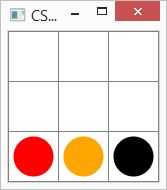
\includegraphics[width=0.16\textwidth]{m-1-3.JPG}}
\subfigure[step 1]{
\label{m-1-0} %% label for second subfigure
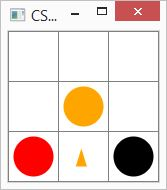
\includegraphics[width=0.16\textwidth]{m-1-0.JPG}}
\subfigure[step 2]{
\label{m-1-1} %% label for second subfigure
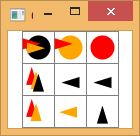
\includegraphics[width=0.16\textwidth]{m-1-1.JPG}}
\subfigure[step 3]{
\label{m-1-2} %% label for second subfigure
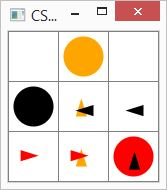
\includegraphics[width=0.16\textwidth]{m-1-2.JPG}}
\subfigure[end]{
\label{m-1-4} %% label for second subfigure
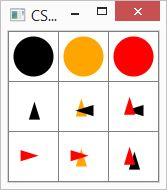
\includegraphics[width=0.16\textwidth]{m-1-4.JPG}}
\caption{Demo of shifting 3 robots}
\label{m-1} %% label for entire figure
\end{figure*}

\begin{figure*}[!t]
% ensure that we have normalsize text
\normalsize
% Store the current equation number.
% Set the equation number to one less than the one
% desired for the first equation here.
% The value here will have to changed if equations
% are added or removed prior to the place these
% equations are referenced in the main text.
\centering
\subfigure[start]{
\label{m-2-0} %% label for first subfigure
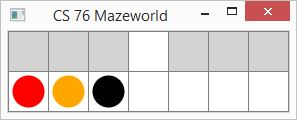
\includegraphics[width=0.18\textwidth]{m-2-0.JPG}}
\subfigure[step 1]{
\label{m-2-0} %% label for first subfigure
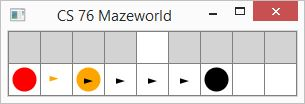
\includegraphics[width=0.18\textwidth]{m-2-1.JPG}}
\subfigure[step 2]{
\label{m-2-0} %% label for first subfigure
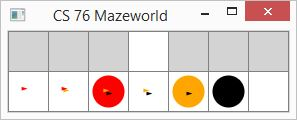
\includegraphics[width=0.18\textwidth]{m-2-2.JPG}}
\subfigure[step 3]{
\label{m-2-0} %% label for first subfigure
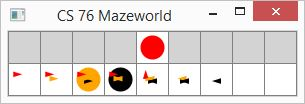
\includegraphics[width=0.18\textwidth]{m-2-3.JPG}}
\subfigure[step 4]{
\label{m-2-0} %% label for first subfigure
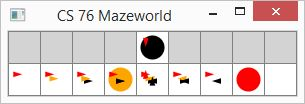
\includegraphics[width=0.18\textwidth]{m-2-4.JPG}}
\subfigure[step 5]{
\label{m-2-0} %% label for first subfigure
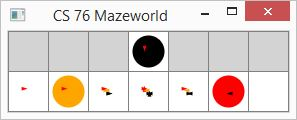
\includegraphics[width=0.18\textwidth]{m-2-5.JPG}}
\subfigure[step 6]{
\label{m-2-0} %% label for first subfigure
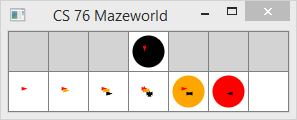
\includegraphics[width=0.18\textwidth]{m-2-6.JPG}}
\subfigure[end]{
\label{m-2-0} %% label for first subfigure
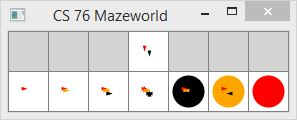
\includegraphics[width=0.18\textwidth]{m-2-7.JPG}}
\caption{Demo of reodering robot in narrow corridor}
\label{m-2} %% label for entire figure
\end{figure*}

\begin{figure*}[!t]
% ensure that we have normalsize text
\normalsize
% Store the current equation number.
% Set the equation number to one less than the one
% desired for the first equation here.
% The value here will have to changed if equations
% are added or removed prior to the place these
% equations are referenced in the main text.
\centering
\subfigure[start]{
\label{m-2-0} %% label for first subfigure
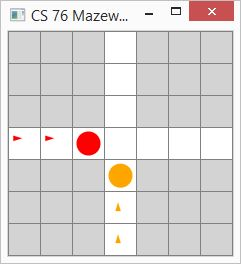
\includegraphics[width=0.18\textwidth]{m-3-0.JPG}}
\subfigure[step 1]{
\label{m-2-0} %% label for first subfigure
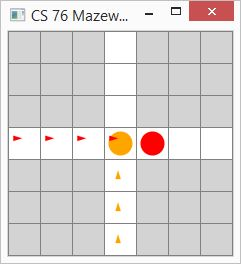
\includegraphics[width=0.18\textwidth]{m-3-1.JPG}}
\subfigure[end]{
\label{m-2-0} %% label for first subfigure
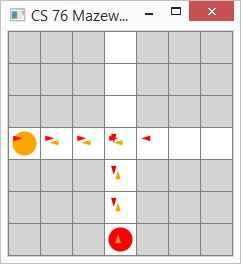
\includegraphics[width=0.18\textwidth]{m-3-2.JPG}}
\caption{Demo of cross road conflict}
\label{m-3} %% label for entire figure
\end{figure*}

\begin{figure*}[!t]
% ensure that we have normalsize text
\normalsize
% Store the current equation number.
% Set the equation number to one less than the one
% desired for the first equation here.
% The value here will have to changed if equations
% are added or removed prior to the place these
% equations are referenced in the main text.
\centering
\subfigure[start]{
\label{m-2-0} %% label for first subfigure
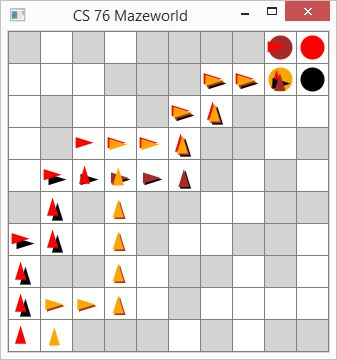
\includegraphics[width=0.618\textwidth]{m-4-1.JPG}}
\caption{Demo of moving relatively large number of robots}
\label{m-4} %% label for entire figure
\end{figure*}

\begin{figure*}[!t]
% ensure that we have normalsize text
\normalsize
% Store the current equation number.
% Set the equation number to one less than the one
% desired for the first equation here.
% The value here will have to changed if equations
% are added or removed prior to the place these
% equations are referenced in the main text.
\centering
\subfigure[start]{
\label{m-2-0} %% label for first subfigure
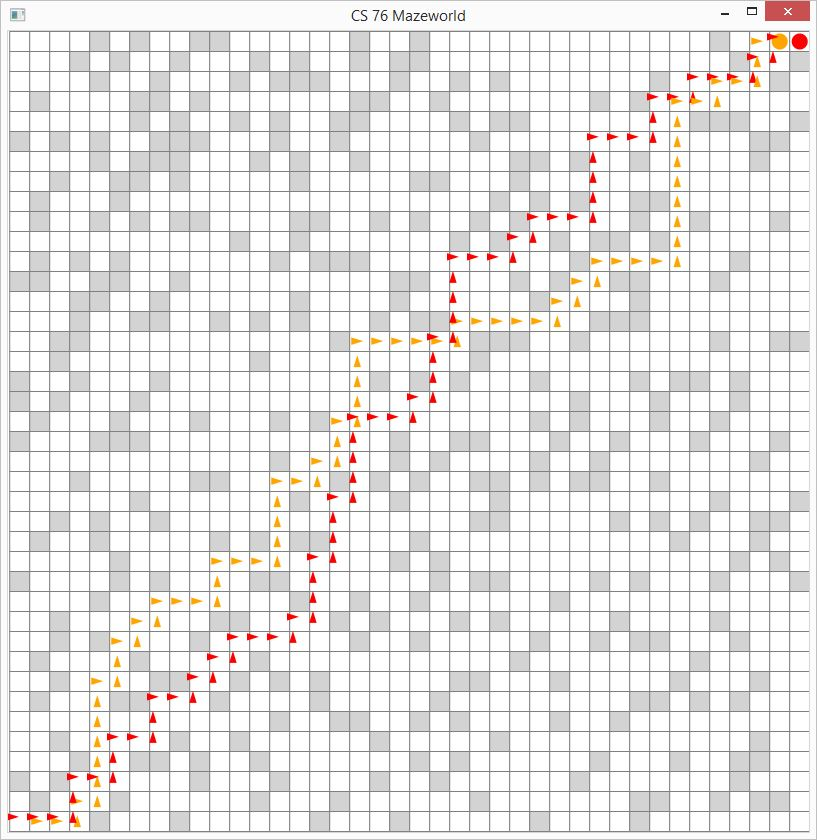
\includegraphics[width=0.818\textwidth]{m-5-1.JPG}}
\caption{Demo of moving relatively large large maze}
\label{m-5} %% label for entire figure
\end{figure*}






\clearpage
\section{Blind robot planning}
\subsection{Problem definition and states}

The basic idea is fill the maze with robots, give them instruction simultaneously, while gradually merging them to one point, which is the goal point.

The initial state looks similar to multi robot problem, which is also a 2-D matrix. $k$ equals to number of cell that is not wall.

$$\begin{pmatrix}
x_0 & y_0 \\
x_1 & y_1 \\
\vdots & \vdots \\	
x_{k-1} & y_{k-1}
\end{pmatrix}$$

The key of the problem is to design a consistent heuristic funciton. Which satisfy the formula in previous section. My intuition is approaching the goal while shrinking the range of robot positions. I think calculating the average and standard deviation of all the coordinates is a reasonable approach. The average describe the center of the group, the deviation describes the convergence. 

So, the state of this problem is as following, noted that $[x_i,y_i]$ and \textbf{c} are $1\times 2$ matrixs :
$$\textbf{c}_{x,y} = \sum^{k-1}_{i=0}[x_i,y_i]/k$$
$$d_{x,y} = ||\sqrt{ \textbf{c}_{x^2,y^2} - (\textbf{c}_{x,y})^2}||$$

Then, the heuristic function would be:
$$h =\textbf{max}(manhattan(\textbf{c}_{x,y}, g_{x,y}), d_{x,y})$$

How do I prove that the heuristic function is consistent? First, it apparently satisfy $h(G)=0$, because at that point, all robot will stay at one point, which makes $ d_{x,y} = 0$. Since the point is the goal, which makes, $manhattan(c_{x,y})=0$. As for $h(N) \leq c(N,P)+h(P) $, it is similar to the way that I used to prove monotonic previously. First let's assume an extreme case where there is an empty $N \times N$ maze, and the goal is at the top-right. I do a little math on it, it seems that if $N > 1 or N < -0.4$, the $cost$ is always larger than $h$. It is obvious always satisfied. (Since I must say I am not a mathematician, I'm not sure if I do it right, feel free to discuss with me if you doubt it).

\subsection{Discussions Polynomial-time blind robot planning}
If we take it as k-robot problem (without collission issue), where $k$ equals to number of cell. Then upper bound of the sates should be $(N)^k$, where N is the free space in maze. Because each of the $k$ robots can occur in any location.

\if
Let's think in antoher way to compute the upper bound of the state space. Assuming the maze is empty, and every robot has its own position at beginning. In k-robot problem, every robot have 4 possible action. So the initial state has 4^k successors. However, in blind robot problem, all the robot move simultaneously with the same action, so there are actually only 4 successors in this problem. Thus the space does not grow exponentially with $k$.
\fi

Assuming the spaces in maze can be desribed by a connected graph. Though the upper bound of space is huge, one big difference from k-robot problem is, the belief state is decreasing, because the robots is merging togethor.  

The problem now is too prove that, if there are 2 robots and moving them simultaneously, can we merge them in polynomial time? If so, We can always pick 2 robot from the $k$ robots, and keep merging the whole states until there is only one left (Actually sometime we merge more than 2 robots at a time).

We can try take actions that trying to shrink their Manhattan distance to 0. How? We can plan a path from A to B, and simply move A to $<x_{B}^{ t = 0}, y_{B}^{ t = 0}>$. Although when A arrive $<x_{B}^{ t = 0}, y_{B}^{ t = 0}>$, B is very likely not there any more, but the Manhattan distance must less or equal than before. The worse case is equal, where B move and A does. But since the map is finite, the Manhattan distance will eventually shorten til 0. It is obvious in a empty maze, wihle a little tricky in a normal maze.

Because Manhattan distance is shrinking at each approaching, the possible state should not be $N^2$ (N is total empty square number, 2 means there are nodes here), but actually less than $N$.

\subsection{Code implementation}

\subsubsection{getSuccessors}
Basic idea of \textbf{getSuccessors} is to move all robots with one action simultaneously. If there is obstacle for a robot, simply not moves. Note that at  \textbf{line 14}, the cost is the amount of robots that moves.
\begin{lstlisting}[numbers=left]
public ArrayList<SearchNode> getSuccessors() {
  ArrayList<SearchNode> successors = new ArrayList<SearchNode>();
  for (int[] action : actions) {
    HashSet<Coordinate> newCoords = new HashSet<>();
    // move all the node in the belief set to direction dxdy
    Coordinate dxdy = new Coordinate(action[0], action[1]);
    for (Coordinate xy : this.allCoord) {
      if (maze.isLegal(xy.x + dxdy.x, xy.y + dxdy.y)) {
        newCoords.add(new Coordinate(xy.x + dxdy.x, xy.y
            + dxdy.y));
      } else {
        // if not legal, simply not moving
        newCoords.add(new Coordinate(xy.x, xy.y));
      }
    }
    successors.add(new BlindRobotNode(newCoords, getCost() + 1.0
        * newCoords.size()));
  }
  return successors;
}
\end{lstlisting}


\subsubsection{Constructors}
The constructor is fairly simple. Note that, \textbf{line 14} is a very important methods, which is used to calculate the average cetner and deviation of all the coordinates. Some one might ask me why don't I compute the average and deviation while adding each new coordinate in the \textbf{getSuccessors}, so that everything can be done in one loop.  I got two reaons here. One is the time complexity is the same. The second is I want to keep the code simple, clean and modular. It is not just more easy to read and maintain, but also benifitial to the computing in the low level, since CPU don't have to access different address frequently.

Noted that the number of existing coordinate is decreasing, since some robots may merge together.
\begin{lstlisting}[numbers=left]
public BlindRobotNode(HashSet<Coordinate> coords, double c) {
  // initiate the positions
  allCoord = coords;
  cost = c;
  newCenDev();
}

// dev = E(x^2) - (Ex)^2
private void newCenDev() {
  center = new Coordinate(0, 0);
  sDeviation = new Coordinate(0, 0);
  for (Coordinate xy : allCoord) {
    center.x += xy.x;
    center.y += xy.y;
    sDeviation.x += Math.pow(xy.x, 2);
    sDeviation.y += Math.pow(xy.y, 2);
  }
  center.x /= allCoord.size();
  center.y /= allCoord.size();
  sDeviation.x = Math.pow(sDeviation.x - center.x * center.x, 0.5);
  sDeviation.y = Math.pow(sDeviation.y - center.y * center.y, 0.5);
}
\end{lstlisting}

\subsubsection{Other methods}



The \textbf{heuristic} method.
\begin{lstlisting}[numbers=left]
@Override
public double heuristic() {
  double dx = coordGoal.x - center.x;
  double dy = coordGoal.y - center.y;
  return Math.max((Math.abs(dx) + Math.abs(dy)),
      (sDeviation.x + sDeviation.y));
}
\end{lstlisting}










\subsection{Output demonstration}

Output of blind robot in 3x3, with the goal at (1,1). (Figure \ref{b-1}):
\begin{lstlisting}[numbers=left]
A*:  
  Nodes explored during search:  15
  Maximum space usage during search 100
  path length: 7
\end{lstlisting}

Output of blind robot in 7x7, with the goal at (3,5). (Figure \ref{b-2}):
\begin{lstlisting}[numbers=left]
A*: 
  Nodes explored during search:  88981
  Maximum space usage during search 622862
  path length: 20
\end{lstlisting}

Output of blind robot in 8x8, with the goal at (0, 0). (Figure \ref{b-3}):
\begin{lstlisting}[numbers=left]
A*: 
  Nodes explored during search:  133773
  Maximum space usage during search 936406
  path length: 23
\end{lstlisting}

\begin{figure*}[!t]
\normalsize
\centering
\subfigure[start]{
\label{b-1-0} %% label for first subfigure
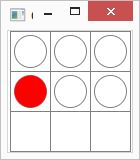
\includegraphics[width=0.18\textwidth]{b-1-2.JPG}}
\subfigure[step 3]{
\label{b-1-0} %% label for first subfigure
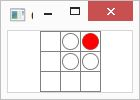
\includegraphics[width=0.18\textwidth]{b-1-3.JPG}}
\subfigure[step 4]{
\label{b-1-0} %% label for first subfigure
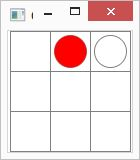
\includegraphics[width=0.18\textwidth]{b-1-4.JPG}}
\subfigure[step 5]{
\label{b-1-0} %% label for first subfigure
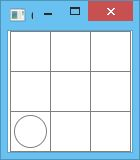
\includegraphics[width=0.18\textwidth]{b-1-5.JPG}}
\subfigure[step 6]{
\label{b-1-0} %% label for first subfigure
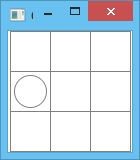
\includegraphics[width=0.18\textwidth]{b-1-6.JPG}}
\subfigure[end]{
\label{b-1-0} %% label for first subfigure
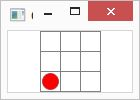
\includegraphics[width=0.18\textwidth]{b-1-7.JPG}}
\caption{Demo of blind robot in 3x3}
\label{b-1} %% label for entire figure
\end{figure*}

\begin{figure*}[!t]
\normalsize
\centering
\subfigure[end]{
\label{b-1-0} %% label for first subfigure
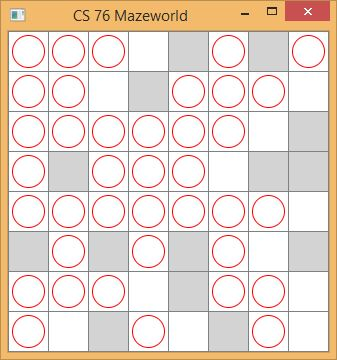
\includegraphics[width=0.309\textwidth]{b-3-1.JPG}}
\caption{Demo of blind robot in 8x8, this time I'm not showing all the snap shot, just want to tell the readers what kind of maze it is.}
\label{b-3} %% label for entire figure
\end{figure*}

\begin{figure*}[!t]
\normalsize
\centering
\subfigure[start]{
\label{b-2-0} %% label for first subfigure
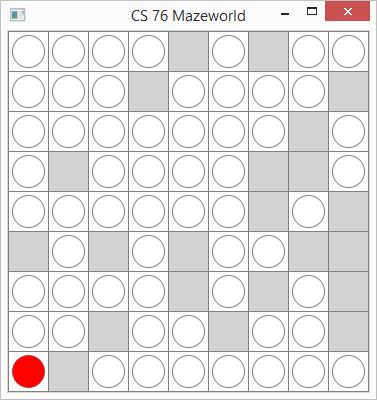
\includegraphics[width=0.18\textwidth]{b-2-1.JPG}}
\subfigure[step 2]{
\label{b-2-0} %% label for first subfigure
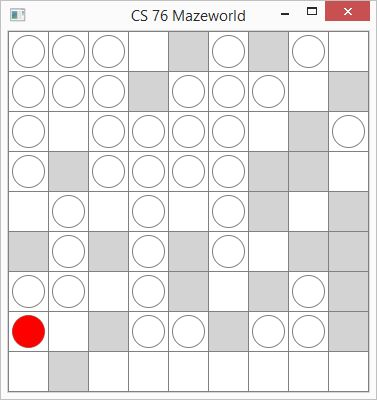
\includegraphics[width=0.18\textwidth]{b-2-2.JPG}}
\subfigure[step 3]{
\label{b-2-0} %% label for first subfigure
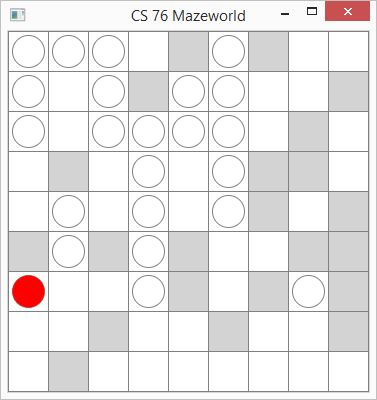
\includegraphics[width=0.18\textwidth]{b-2-3.JPG}}
\subfigure[step 4]{
\label{b-2-0} %% label for first subfigure
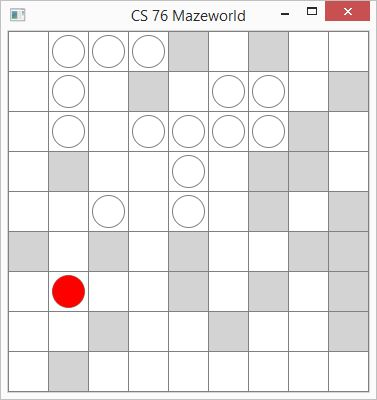
\includegraphics[width=0.18\textwidth]{b-2-4.JPG}}
\subfigure[step 5]{
\label{b-2-0} %% label for first subfigure
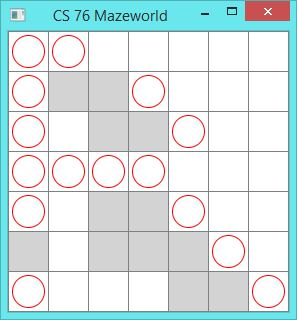
\includegraphics[width=0.18\textwidth]{b-2-5.JPG}}
\subfigure[step 6]{
\label{b-2-0} %% label for first subfigure
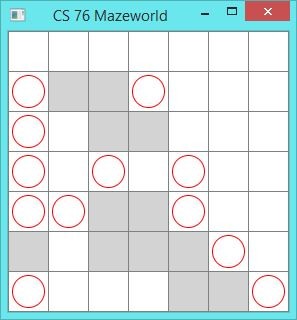
\includegraphics[width=0.18\textwidth]{b-2-6.JPG}}
\subfigure[step 7]{
\label{b-2-0} %% label for first subfigure
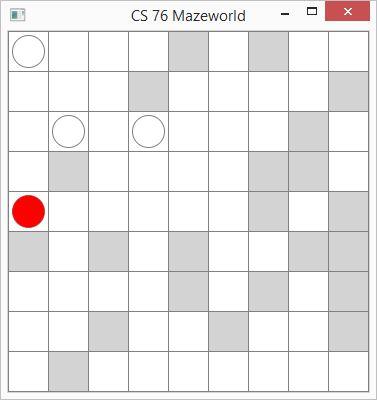
\includegraphics[width=0.18\textwidth]{b-2-7.JPG}}
\subfigure[step 7]{
\label{b-2-0} %% label for first subfigure
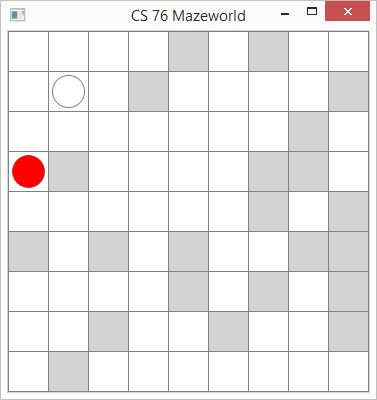
\includegraphics[width=0.18\textwidth]{b-2-8.JPG}}
\subfigure[step 7]{
\label{b-2-0} %% label for first subfigure
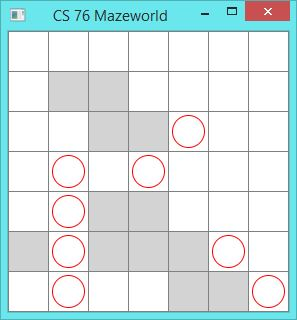
\includegraphics[width=0.18\textwidth]{b-2-9.JPG}}
\subfigure[step 7]{
\label{b-2-0} %% label for first subfigure
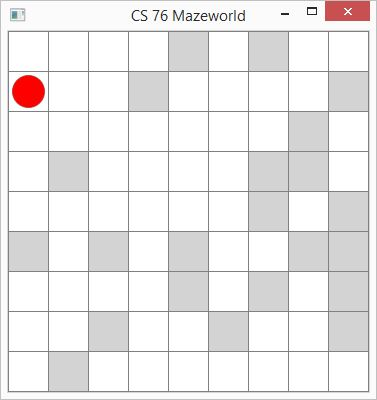
\includegraphics[width=0.18\textwidth]{b-2-10.JPG}}
\subfigure[step 11]{
\label{b-2-0} %% label for first subfigure
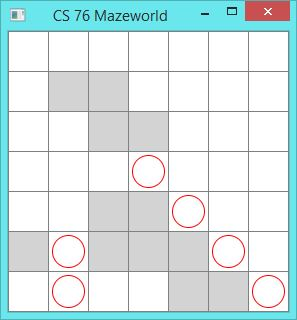
\includegraphics[width=0.18\textwidth]{b-2-11.JPG}}
\subfigure[step 12]{
\label{b-2-0} %% label for first subfigure
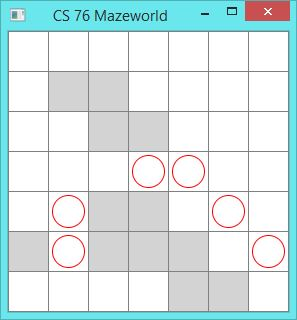
\includegraphics[width=0.18\textwidth]{b-2-12.JPG}}
\subfigure[step 13]{
\label{b-2-0} %% label for first subfigure
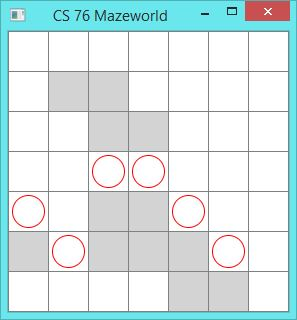
\includegraphics[width=0.18\textwidth]{b-2-13.JPG}}
\subfigure[step 14]{
\label{b-2-0} %% label for first subfigure
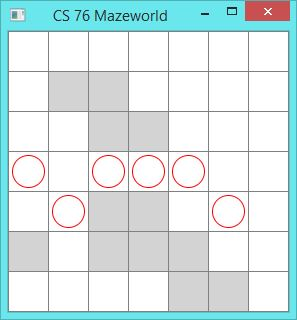
\includegraphics[width=0.18\textwidth]{b-2-14.JPG}}
\subfigure[step 15]{
\label{b-2-0} %% label for first subfigure
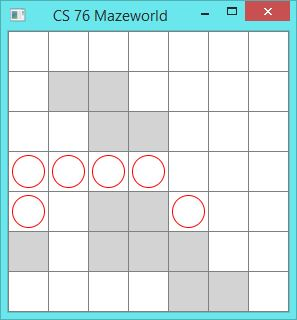
\includegraphics[width=0.18\textwidth]{b-2-15.JPG}}
\subfigure[step 16]{
\label{b-2-0} %% label for first subfigure
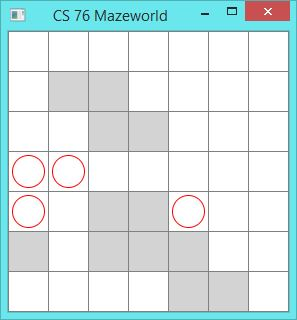
\includegraphics[width=0.18\textwidth]{b-2-16.JPG}}
\subfigure[step 17]{
\label{b-2-0} %% label for first subfigure
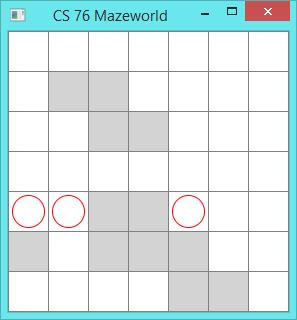
\includegraphics[width=0.18\textwidth]{b-2-17.JPG}}
\subfigure[step 18]{
\label{b-2-0} %% label for first subfigure
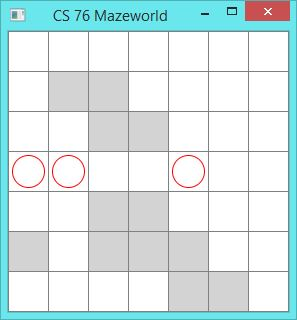
\includegraphics[width=0.18\textwidth]{b-2-18.JPG}}
\subfigure[step 19]{
\label{b-2-0} %% label for first subfigure
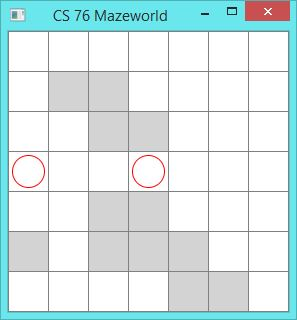
\includegraphics[width=0.18\textwidth]{b-2-19.JPG}}
\subfigure[step 20]{
\label{b-2-0} %% label for first subfigure
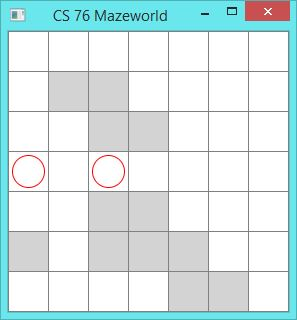
\includegraphics[width=0.18\textwidth]{b-2-20.JPG}}
\subfigure[step 21]{
\label{b-2-0} %% label for first subfigure
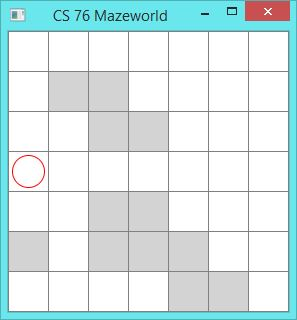
\includegraphics[width=0.18\textwidth]{b-2-21.JPG}}
\subfigure[step 22]{
\label{b-2-0} %% label for first subfigure
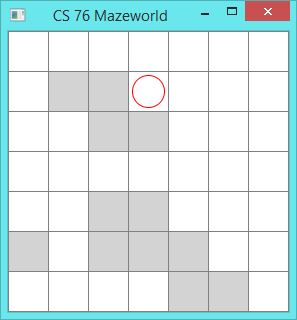
\includegraphics[width=0.18\textwidth]{b-2-22.JPG}}
\caption{Demo of blind robot in 7x7}
\label{b-2} %% label for entire figure
\end{figure*}






\section{Previous work}

For the k-robot problem, one biggest obstacle here is that the state space grow exponentially with the number of robots, which is $N^k$. This article put forward a very efficient method to find the optimal solution quick against the huge states space \footnote{Standley, T. 2010. Finding optimal solutions to cooperative pathfinding problems. In The Twenty-Fourth AAAI Conference on Artificial Intelligence (AAAI’10), 173–178.}.  The philosophy here is, they first A* to plan the shortest path individually. Then they resolve the conflict that occurs in in the $k$ paths. If it cannot be resovled, they merge them in to one group and solve this path as m-robot problem individually. Notice that $m \leq k$. 

In order to face the real time demand, such as gaming system, they further design this method, by incorporating the idea of iterative deepening. While increasing the grouping number from one to some large number, they keep record  of groups with lower bound, which is quite helpful in the latter iteration.

\section{Appendix}
This is the auxiliary class I used to simpilify my codes.
\begin{lstlisting}[numbers=left]
public class Coordinate {
  public Double x;
  public Double y;

  void add2center(Coordinate other, int newN) {
    x = (x * (newN - 1) + other.x) / newN;
    y = (y * (newN - 1) + other.y) / newN;
  }

  Coordinate(int a, int b) {
    x = (double) a;
    y = (double) b;
  }

  Coordinate(double a, double b) {
    x = a;
    y = b;
  }

  Coordinate(Coordinate other) {
    x = other.x;
    y = other.y;
  }

  public int getX() {
    return x.intValue();
  }

  public int getY() {
    return y.intValue();
  }

  private boolean equalWithCast(Object other) {
    return Math.abs((x - ((Coordinate) other).x)) < 0.01
        && (Math.abs(y - ((Coordinate) other).y) < 0.01);
  }

  private boolean isZero() {
    return (x < 0.01) && (y < 0.01);
  }

  @Override
  public boolean equals(Object other) {
    return hashCode() == ((Coordinate) other).hashCode();
  }

  @Override
  public int hashCode() {
    return (int) (x + 1000 * y);
  }

  @Override
  public String toString() {
    DecimalFormat df = new DecimalFormat("0.0");
    return "(" + df.format(x) + "," + df.format(y) + ")";
  }
}
\end{lstlisting}









\end{document}